
\section{Calorimetric Measurements} 
\label{sec:calorimetery} 

To obtain a preliminary characterization of the calorimetric performance 
of the CdTe sensors, we measure the total charge collected out of the CdTe 
sensor for various incident electron beam energies. Examples of the 
charge distributions are shown in Figure~\ref{fig:ChargeDistribution}
for $2$~GeV and $200$~GeV electrons. For electrons with energy between 
$2$~GeV and $7$~GeV, the sensor was placed after $2$ radiation lengths 
of lead absorber, and for electrons with energy above $50$~GeV, the 
sensor was placed after $6$ radiation lengths of three alternating layers of 
tungsten and lead. 

%Fig: Charge distributions (noise, showers, MIP?)
\begin{figure}[htbp] 
\centering
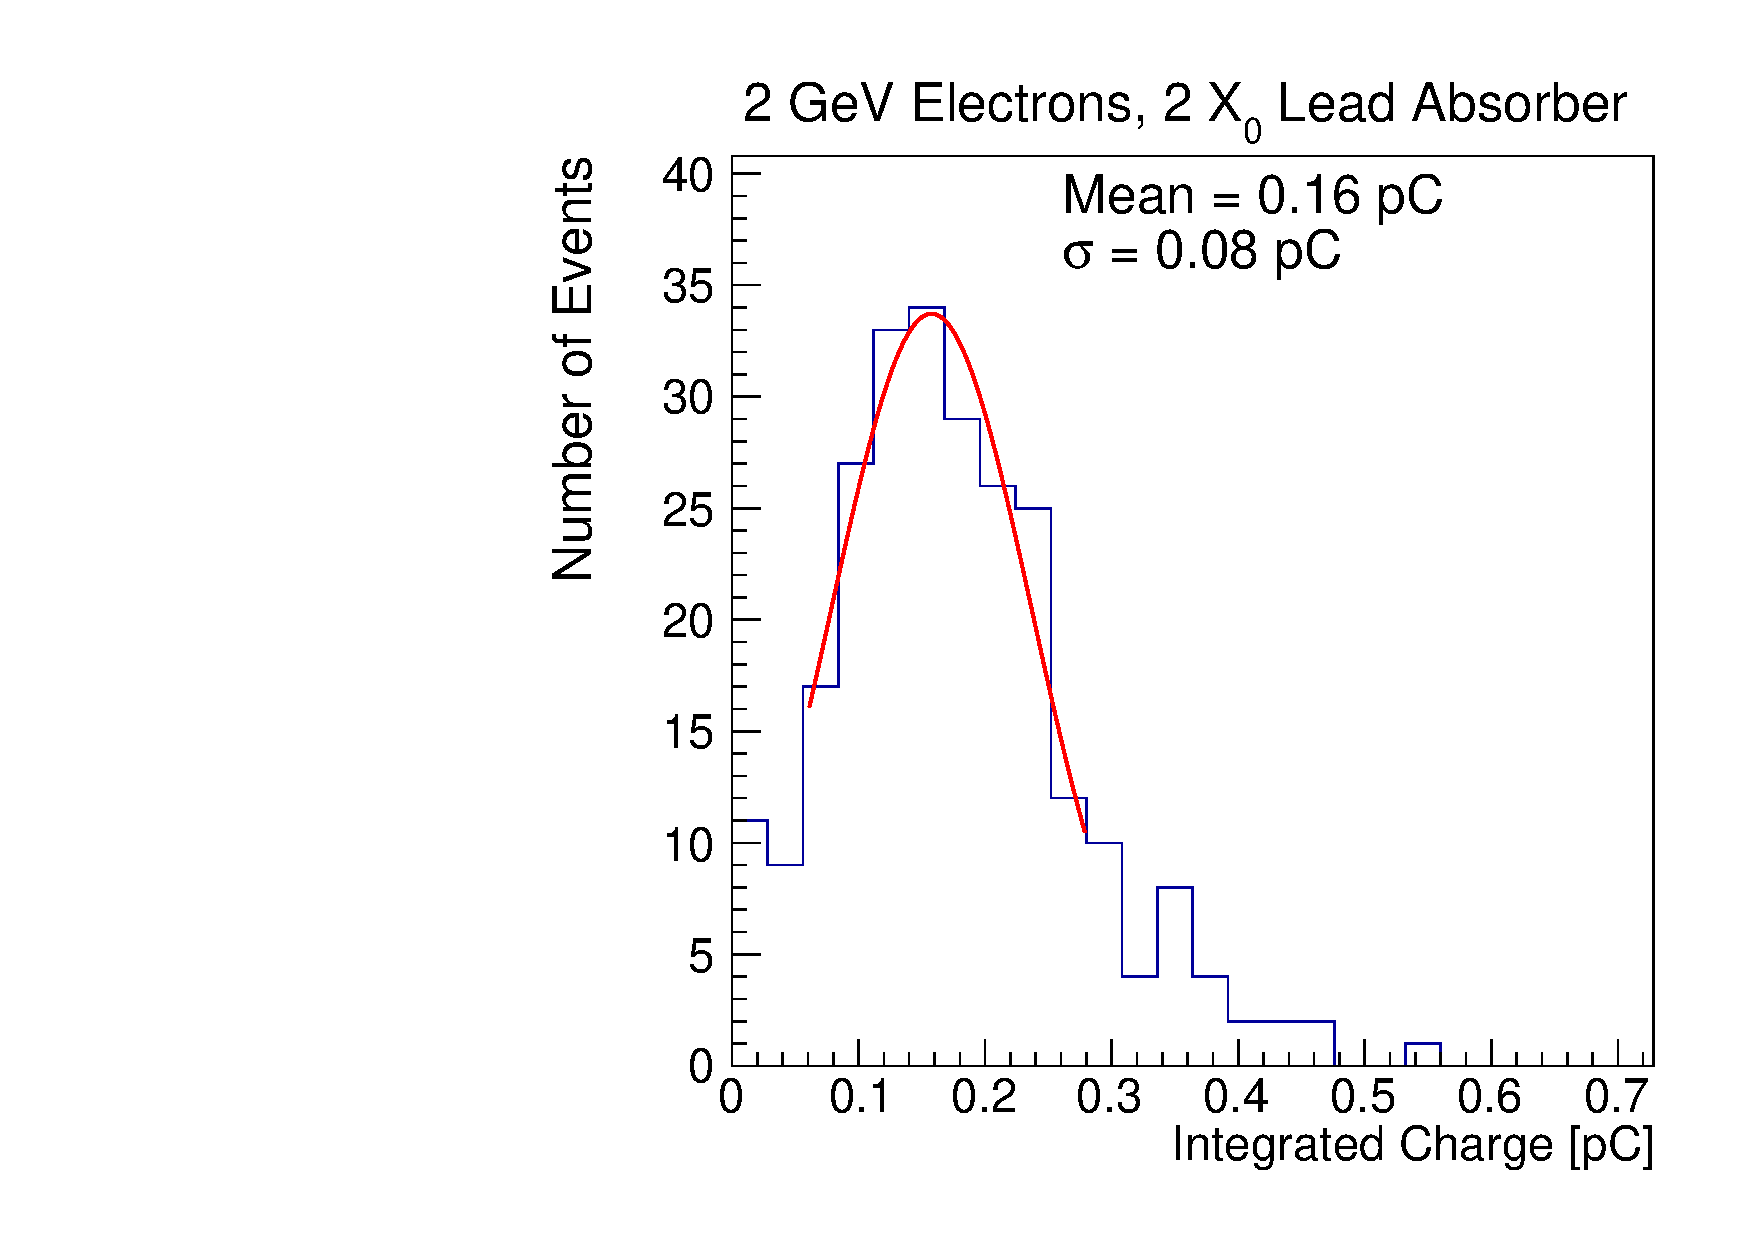
\includegraphics[width=0.49\textwidth]{figures/2GeV_charge.pdf} 
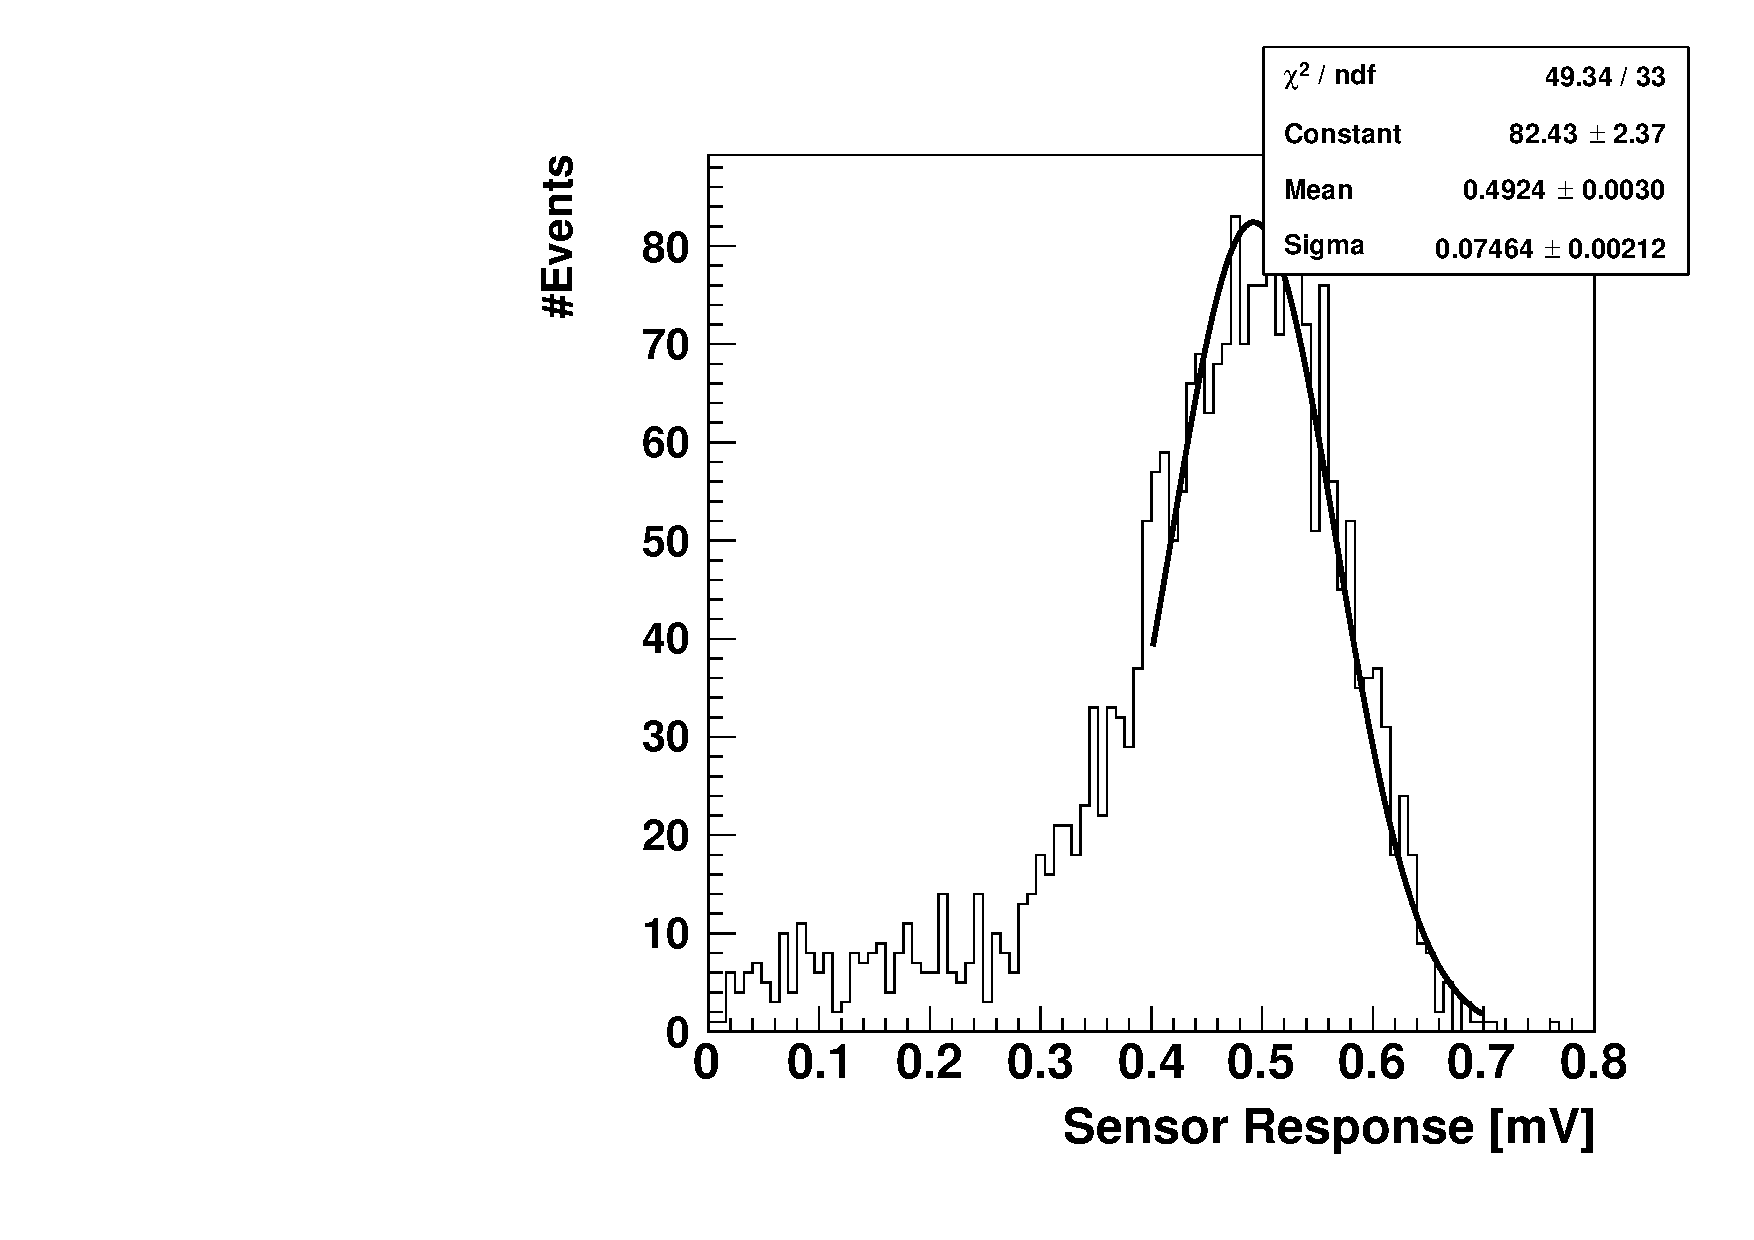
\includegraphics[width=0.49\textwidth]{figures/CdTeEnergy.pdf} 
\caption{Distribution of total charge collected in the CdTe sensor for a $2$~GeV
electron after $2$~$\mathrm{X}_{0}$ of lead absorber (left) and a 100~GeV
electron after $6$~$\mathrm{X}_{0}$ of tungsten and lead absorber (right). The plot
to the right as a fiducial cut with respect to the center of the sensor of $\mathrm{3 \times 3 mm}$ applied to the incidenting electrons.} 
\label{fig:ChargeDistribution} 
\end{figure} 

We plot the mean collected charge as a function of the incident beam energy
in Figure~\ref{fig:ChargeVsEnergy} and observe that the signal size scales
up with increasing beam energy. The resolution is measured as the width
parameter of a Gaussian fit to the charge distribution and is shown by the green bars. 
The measured resolution ranges from
about $50\%$ for electrons in the range of a few GeV to 
about $30\%$ for electrons above $50$~GeV. 
These resolution measurements are encouraging given that they are performed
using only a single layer sample covering a relatively small transverse
geometric area. In future studies, we intend to improve the characterization
of the calorimetric performance by completing measurements of the
longitudinal shower profile and to instrument a larger transverse 
area to improve the transverse shower containment. 

%Fig: Collected Charge vs Beam Energy
\begin{figure}[htbp] 
\centering
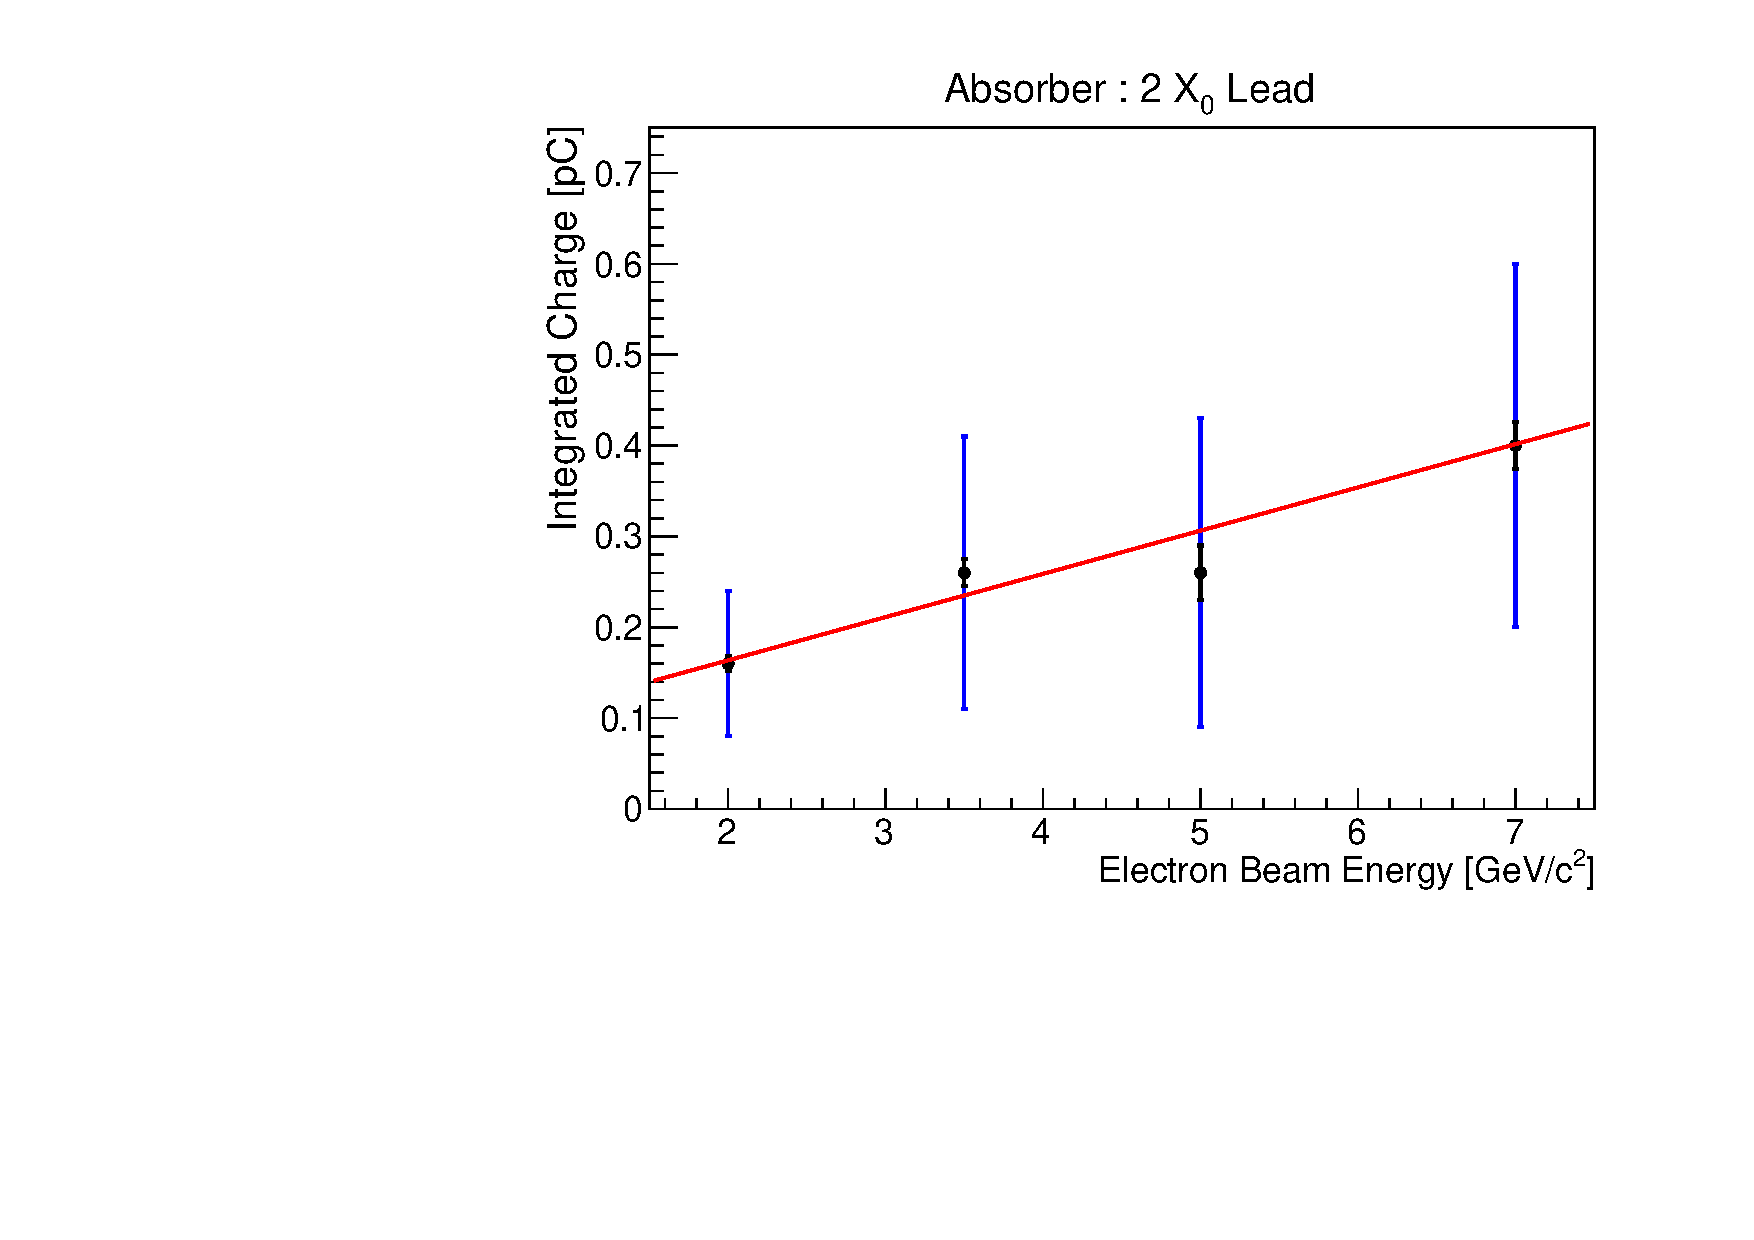
\includegraphics[width=0.49\textwidth]{figures/ChargeVsEnergyAt2X0.pdf} 
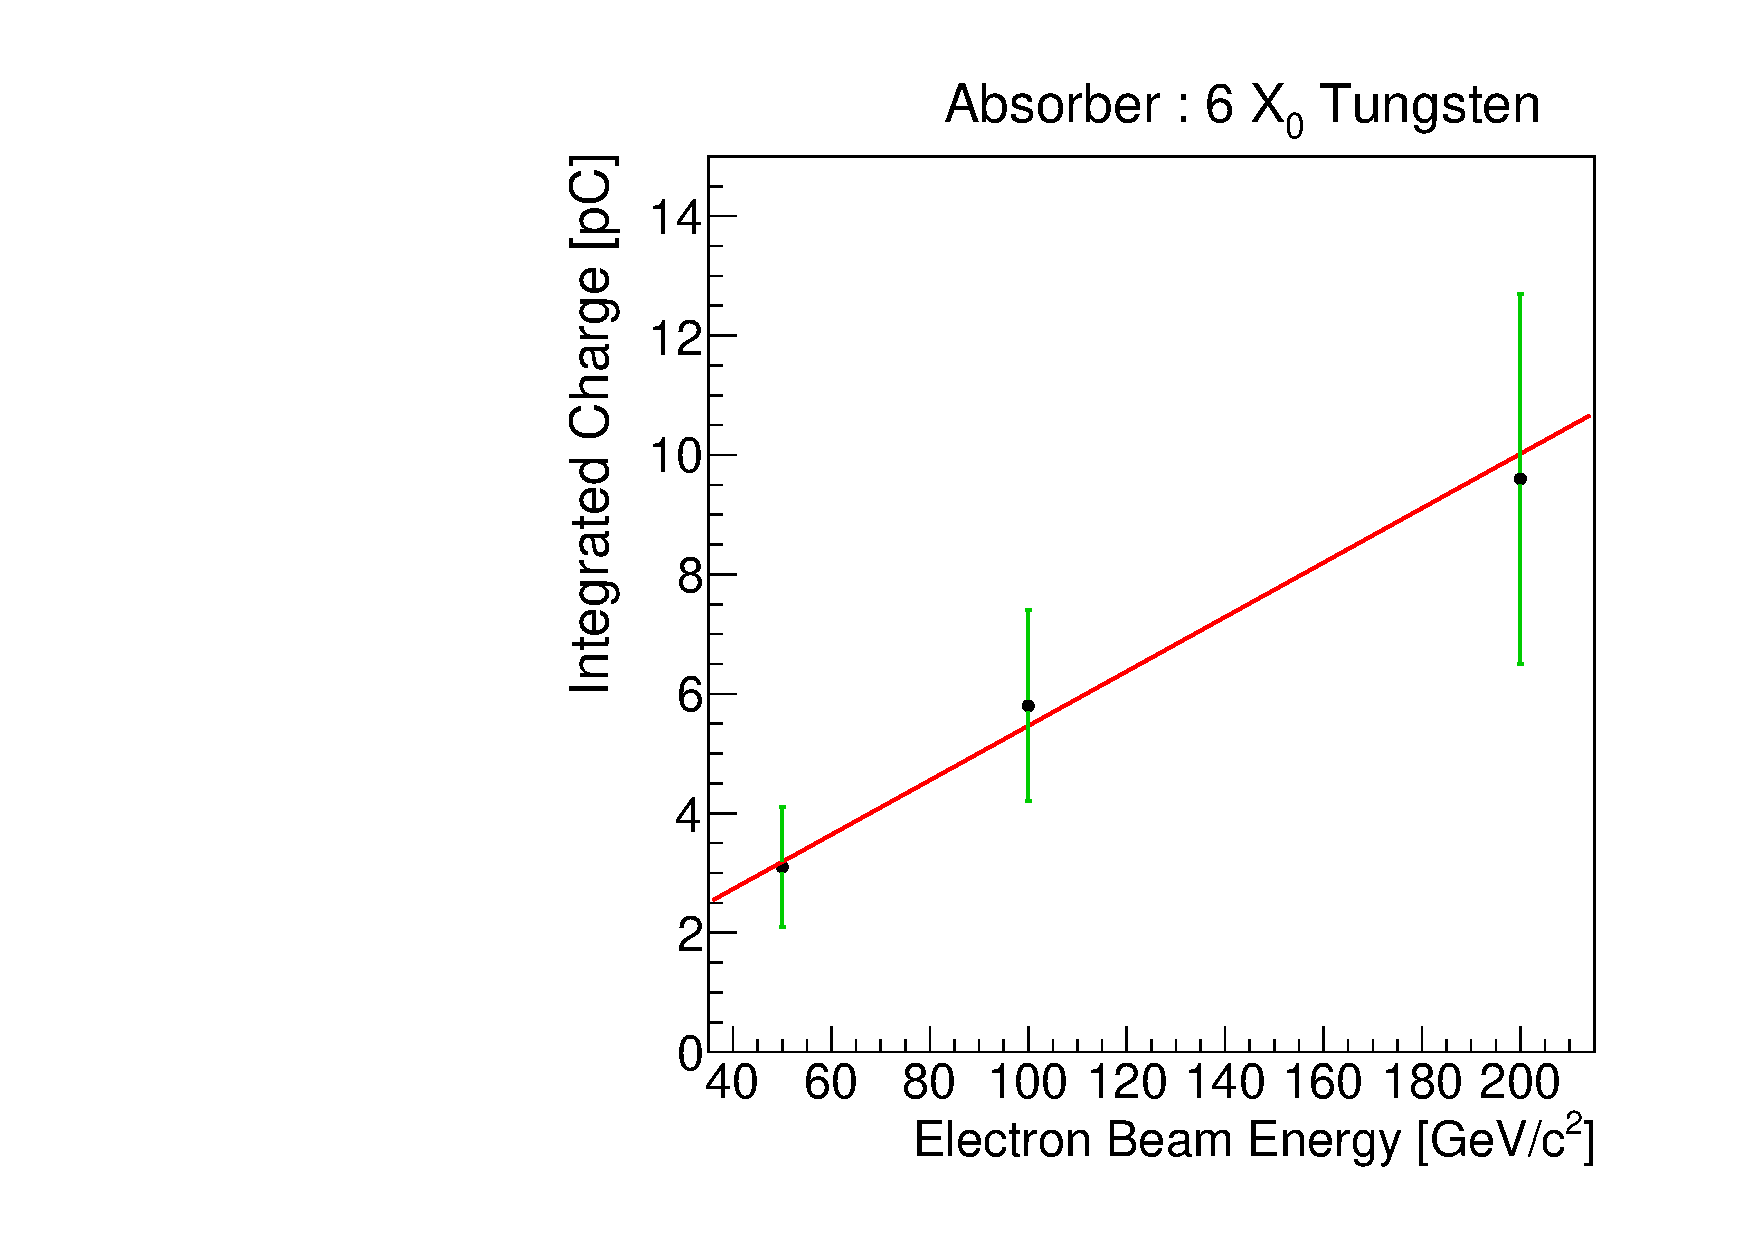
\includegraphics[width=0.49\textwidth]{figures/ChargeVsEnergyAt6X0.pdf} 
\caption{ The mean charge collected in the CdTe sensor is plotted as a function
of the electron beam energy. Left: Measurements performed at the T9 beamline
with $2$~$\mathrm{X}_{0}$ of lead absorber placed directly in front of the 
CeTe sensor. Right: Measurements performed at the H2 beamline
with $6$~$\mathrm{X}_{0}$ of tungsten absorber placed directly in front of the 
CeTe sensor. The blue bars show the uncertainty on the mean integrated charge
extracted from the Gaussian fit to the charge distribution, while the green 
bars show the measured resolution. The red line is a 
linear fit to each set of measured data. } 
\label{fig:ChargeVsEnergy} 
\end{figure} 


